\documentclass[a4paper]{article}
\usepackage[utf8]{inputenc}
\usepackage[russian]{babel}
\usepackage{listings}
\usepackage[a4paper,margin=1.2in]{geometry}
\usepackage{indentfirst}
\usepackage{graphicx}
\usepackage{caption}
\usepackage{float}

%\setcounter{topnumber}{2}
%\setcounter{bottomnumber}{2}
%\setcounter{totalnumber}{4}
%\renewcommand{\topfraction}{0.85}
%\renewcommand{\bottomfraction}{0.85}
%\renewcommand{\textfraction}{0.15}
%\renewcommand{\floatpagefraction}{0.8}
%\renewcommand{\textfraction}{0.1}
%\setlength{\floatsep}{5pt plus 2pt minus 2pt}
%\setlength{\textfloatsep}{5pt plus 2pt minus 2pt}
%\setlength{\intextsep}{5pt plus 2pt minus 2pt}

\begin{document}

\title{Сравнение методов глобальной оптимизации на нескольких классах тестовых задач}
\author{}
\date{}
\maketitle

\section{Список алгоритмов}
\begin{itemize}
  \item Алгоритм глобального поиска (AGS)
  \item Multi Level Single Linkage (MLSL)
  \item DIRECT
  \item Locally-based DIRECT (DIRECT$l$)
  \item Dual Simulated Annealing
  \item Differential Evolution
  \item Controlled Random Search
  \item Simple
\end{itemize}

\section{Результаты на классе задач $F_{GR}$}

\begin{figure}[H]
  \center
  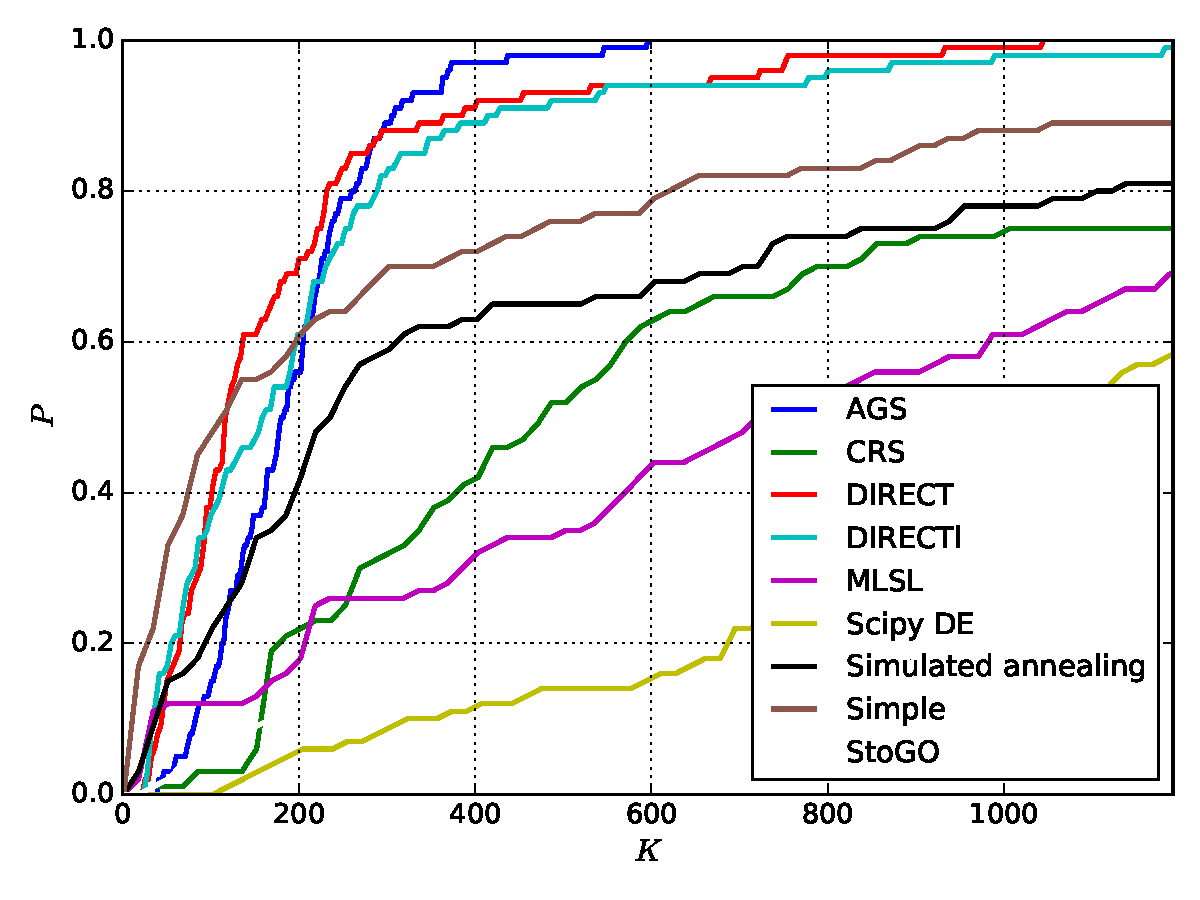
\includegraphics[width=0.95\textwidth]{../experiments/grish/cmc.pdf}
  \caption{Остановка после попадания в окрестность размера $10^{-2}$}
  \label{fig:}
\end{figure}

\section{Результаты на классах задач $GKLS$ различной размерности}

\begin{figure}[H]
  \center
  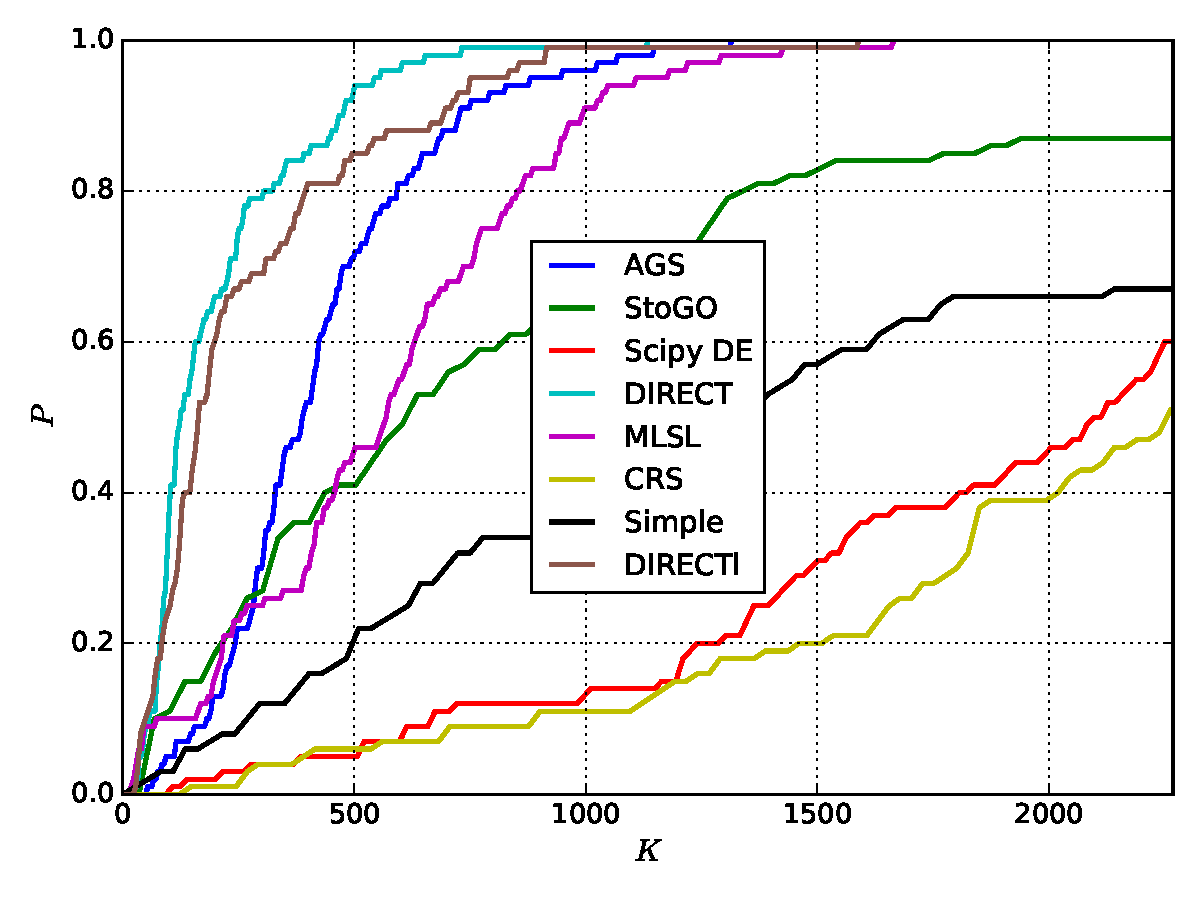
\includegraphics[width=0.95\textwidth]{../experiments/gklss2d/cmc.pdf}
  \caption{Класс GKLS Simple 2d. Остановка после попадания в окрестность размера $2\cdot10^{-2}$}
  \label{fig:}
\end{figure}

\begin{figure}[H]
  \center
  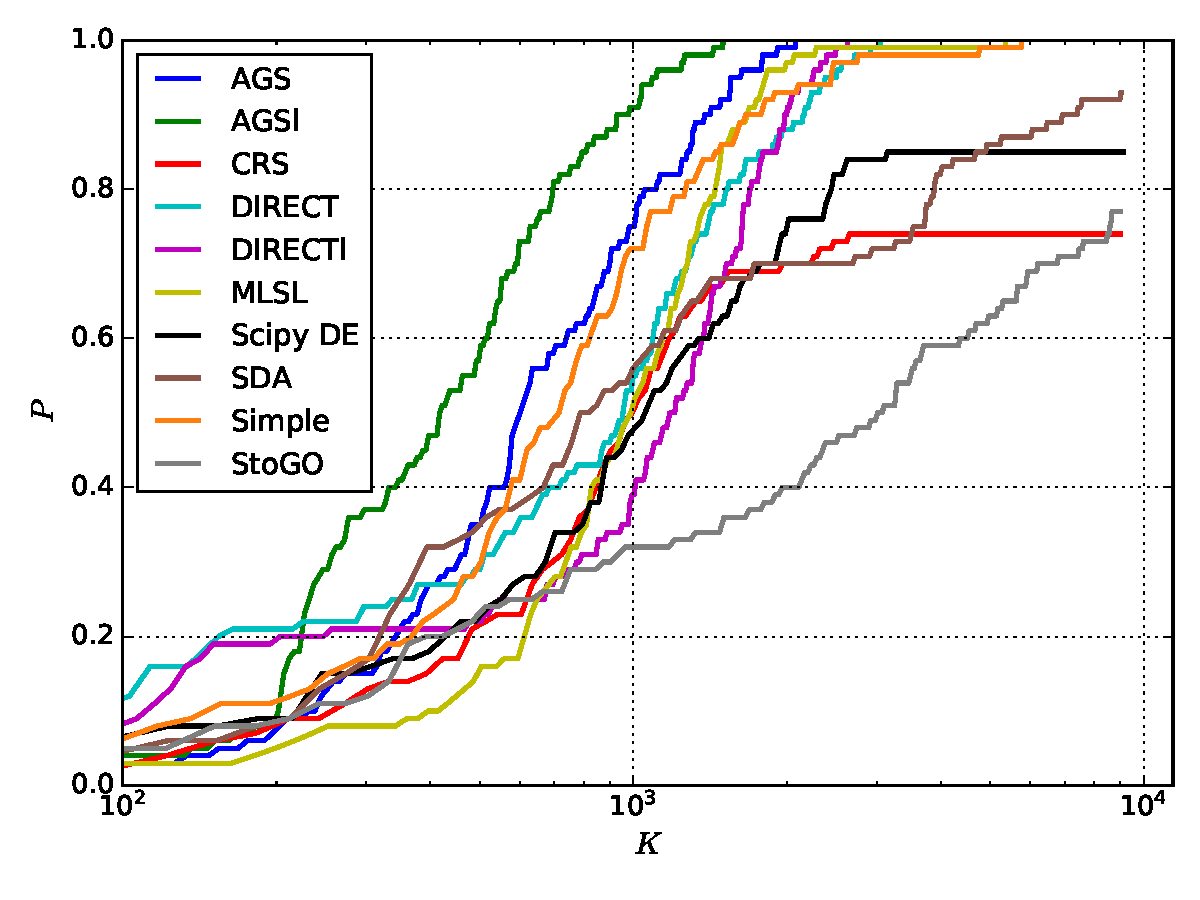
\includegraphics[width=0.95\textwidth]{../experiments/gklsh2d/cmc.pdf}
  \caption{Класс GKLS Hard 2d. Остановка после попадания в окрестность размера $2\cdot10^{-2}$}
  \label{fig:}
\end{figure}

\begin{figure}[H]
  \center
  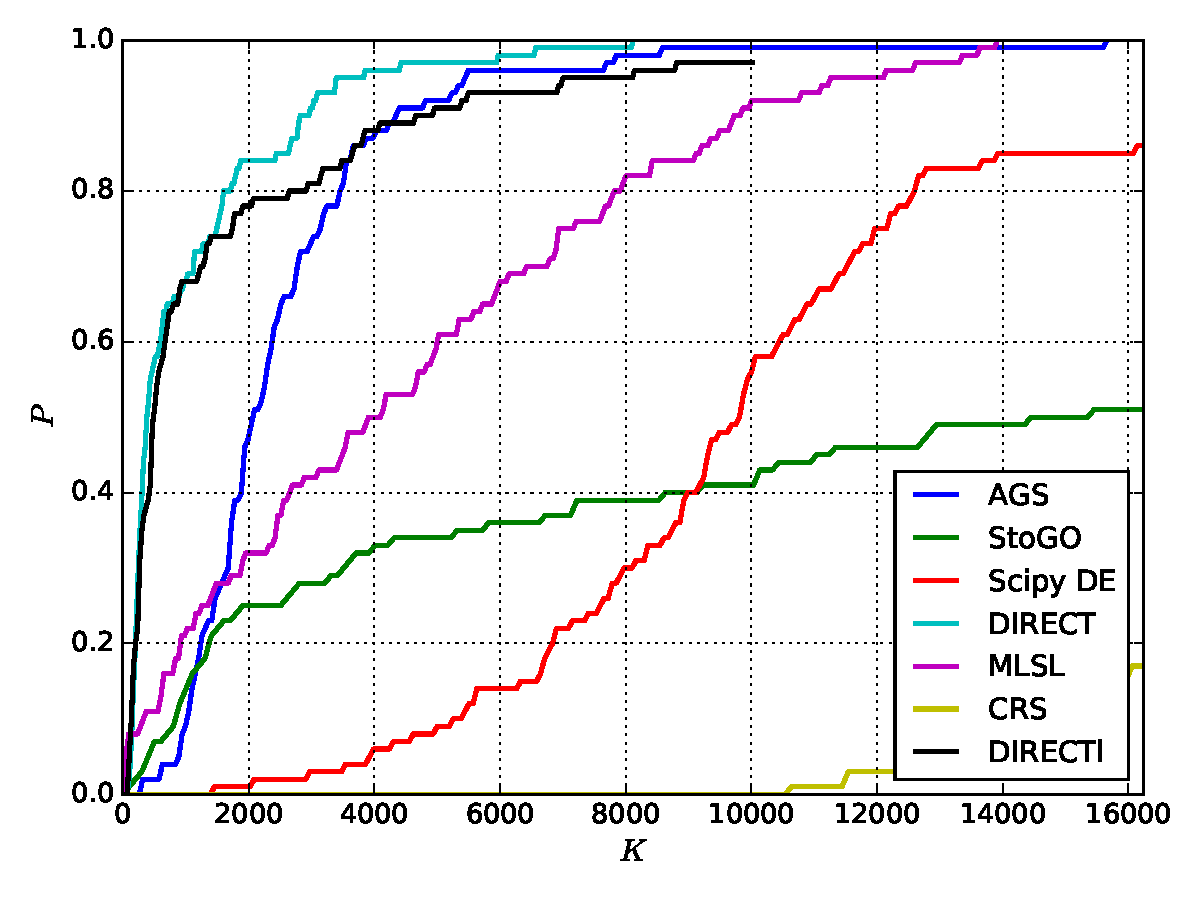
\includegraphics[width=0.95\textwidth]{../experiments/gklss3d/cmc.pdf}
  \caption{Класс GKLS Simple 3d. Остановка после попадания в окрестность размера $2\cdot10^{-2}$}
  \label{fig:}
\end{figure}

\begin{figure}[H]
  \center
  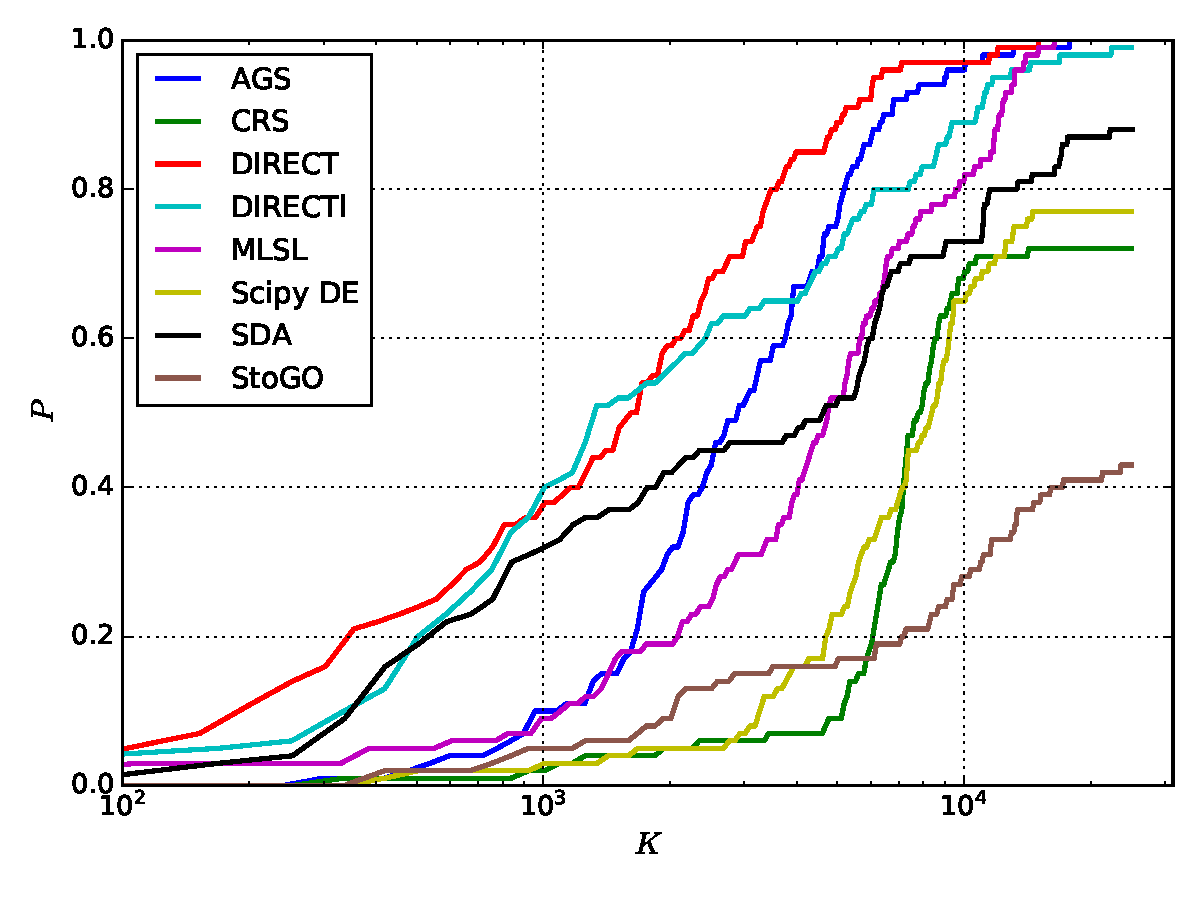
\includegraphics[width=0.95\textwidth]{../experiments/gklsh3d/cmc.pdf}
  \caption{Класс GKLS Hard 3d. Остановка после попадания в окрестность размера $2\cdot10^{-2}$}
  \label{fig:}
\end{figure}

\begin{figure}[H]
  \center
  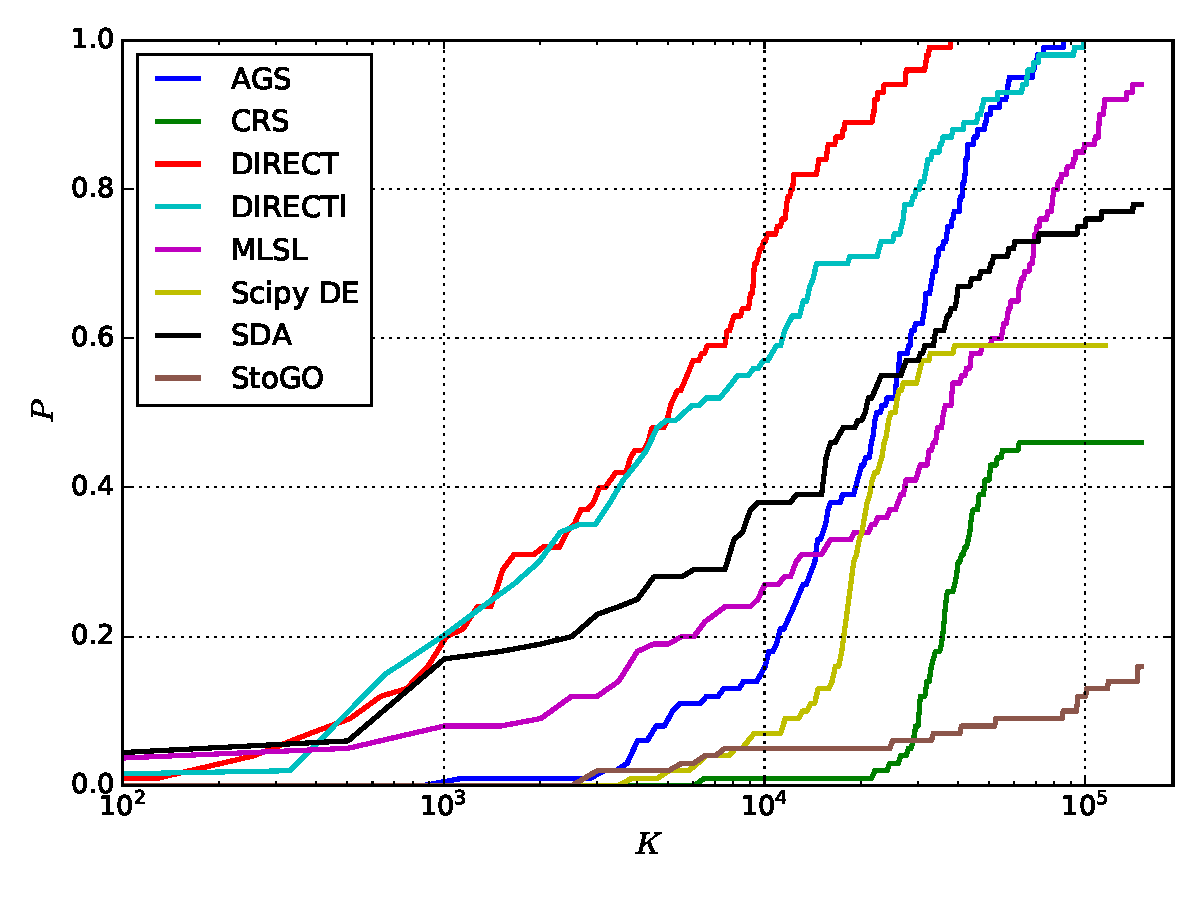
\includegraphics[width=0.95\textwidth]{../experiments/gklss4d/cmc.pdf}
  \caption{Класс GKLS Simple 4d. Остановка после попадания в окрестность размера $2\cdot10^{-2}$}
  \label{fig:}
\end{figure}

\begin{figure}[H]
  \center
  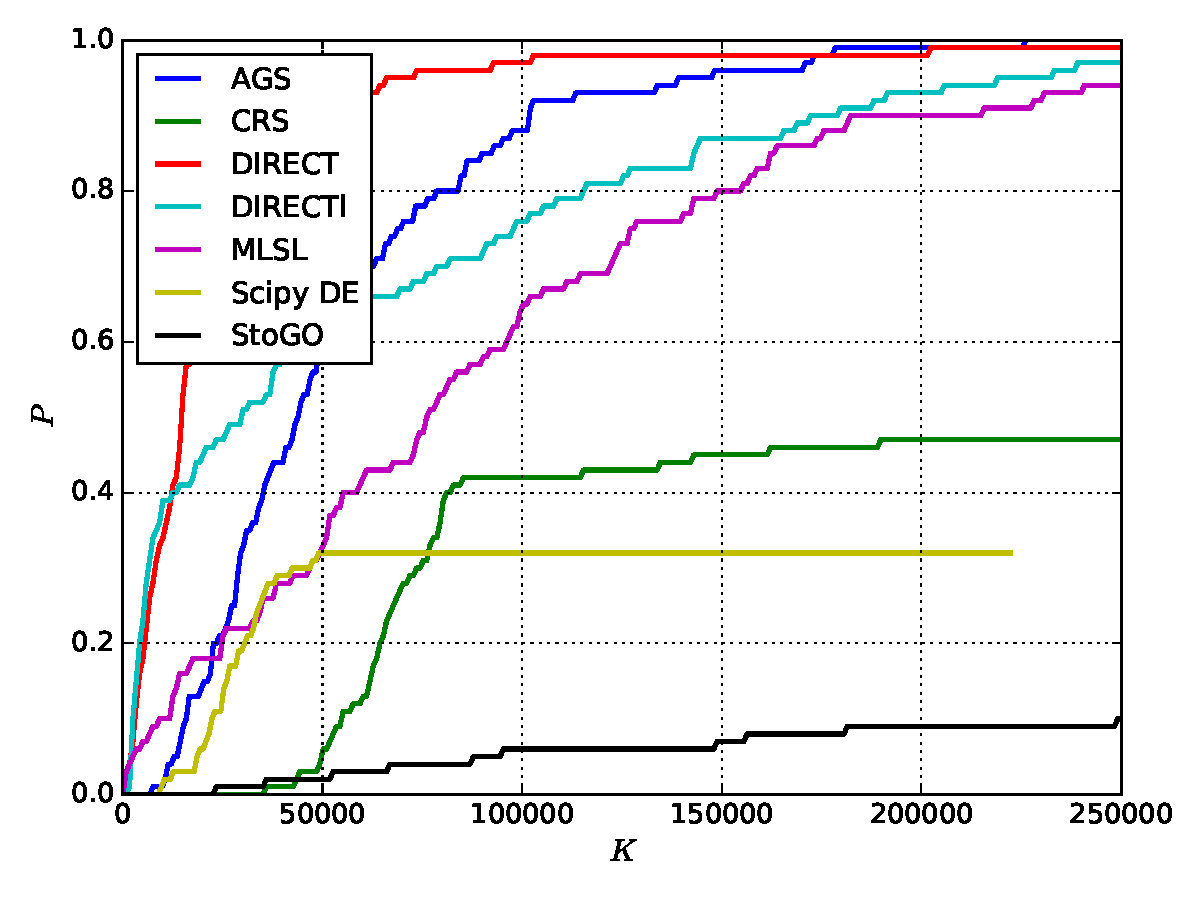
\includegraphics[width=0.95\textwidth]{../experiments/gklsh4d/cmc.pdf}
  \caption{Класс GKLS Hard 4d. Остановка после попадания в окрестность размера $2\cdot10^{-2}$}
  \label{fig:}
\end{figure}

\begin{figure}[H]
  \center
  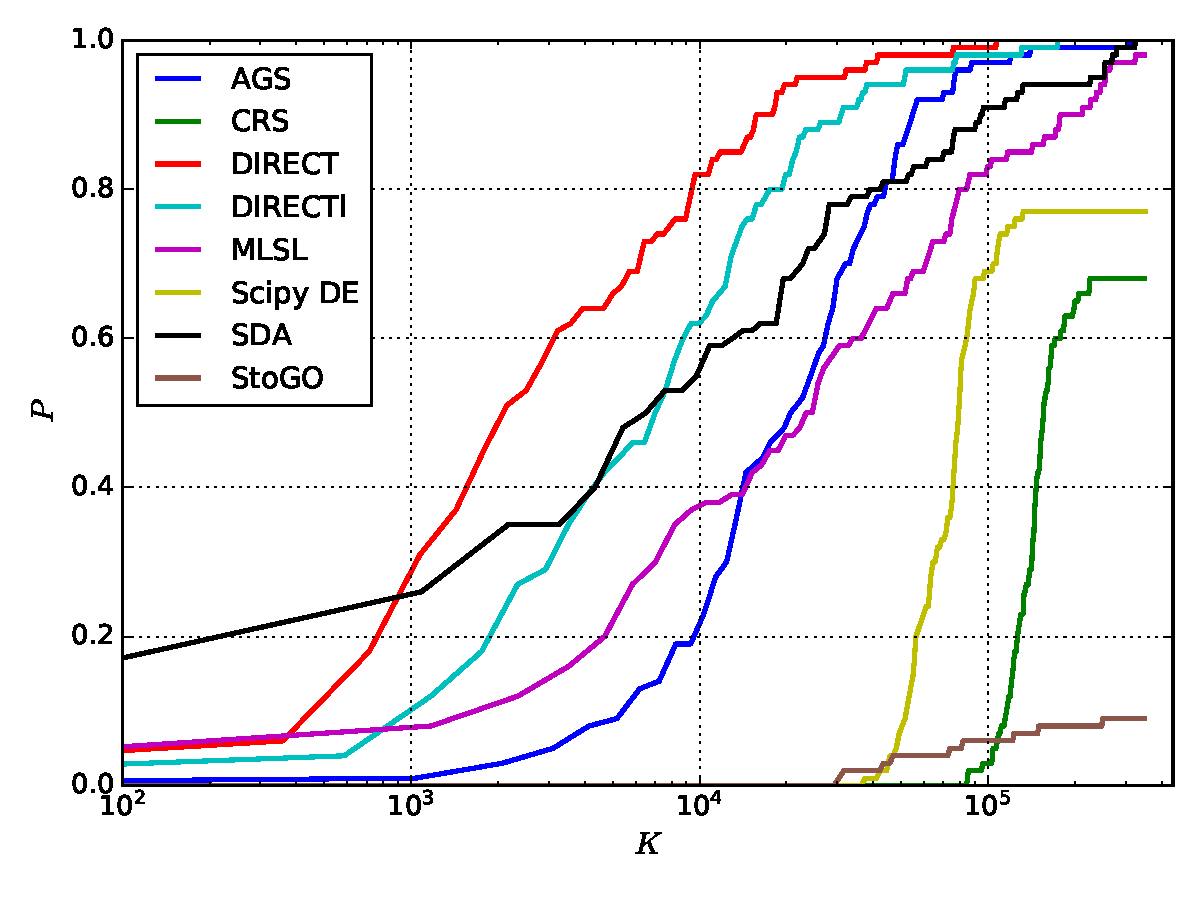
\includegraphics[width=0.95\textwidth]{../experiments/gklss5d/cmc.pdf}
  \caption{Класс GKLS Simple 5d. Остановка после попадания в окрестность размера $2\cdot10^{-2}$}
  \label{fig:}
\end{figure}

\begin{figure}[H]
  \center
  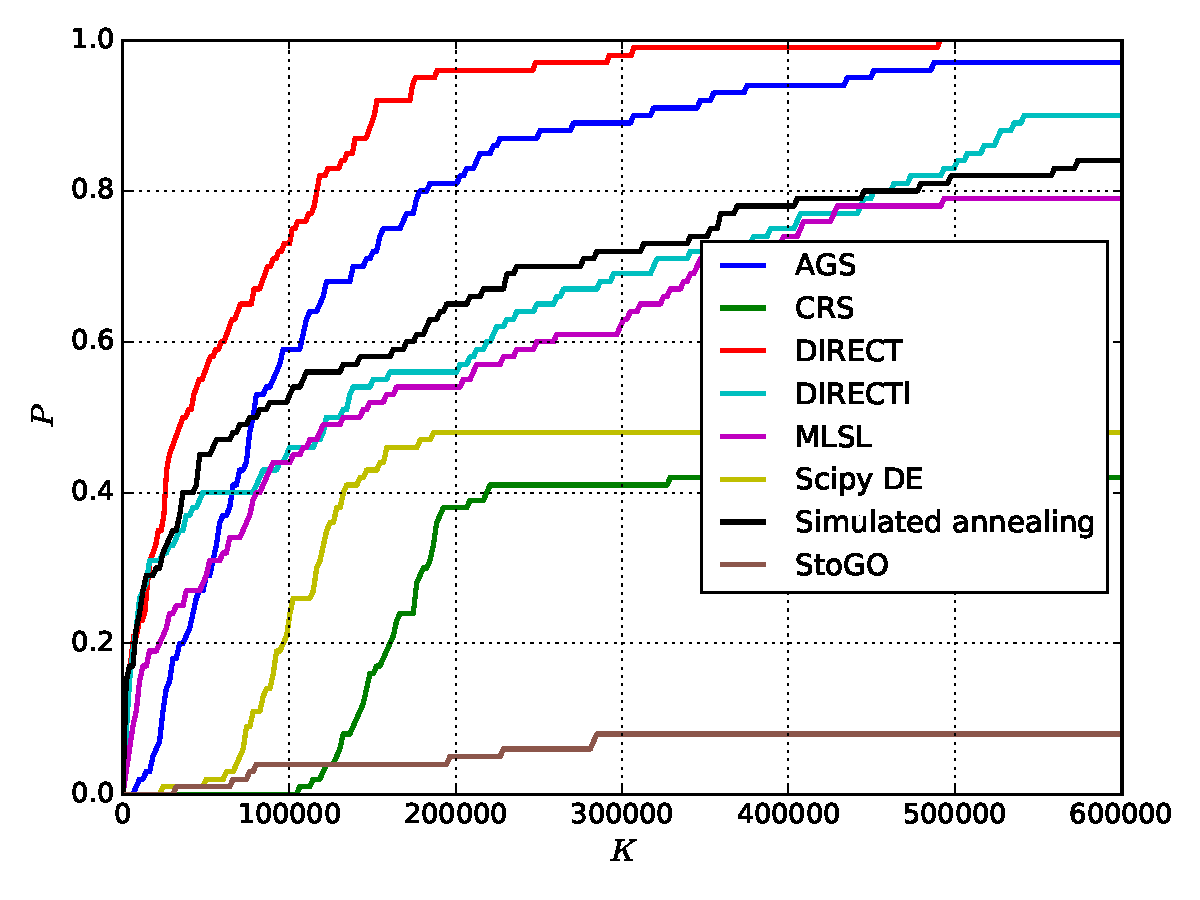
\includegraphics[width=0.95\textwidth]{../experiments/gklsh5d/cmc.pdf}
  \caption{Класс GKLS Hard 5d. Остановка после попадания в окрестность размера $2\cdot10^{-2}$}
  \label{fig:}
\end{figure}


\begin{figure}[H]
  \center
  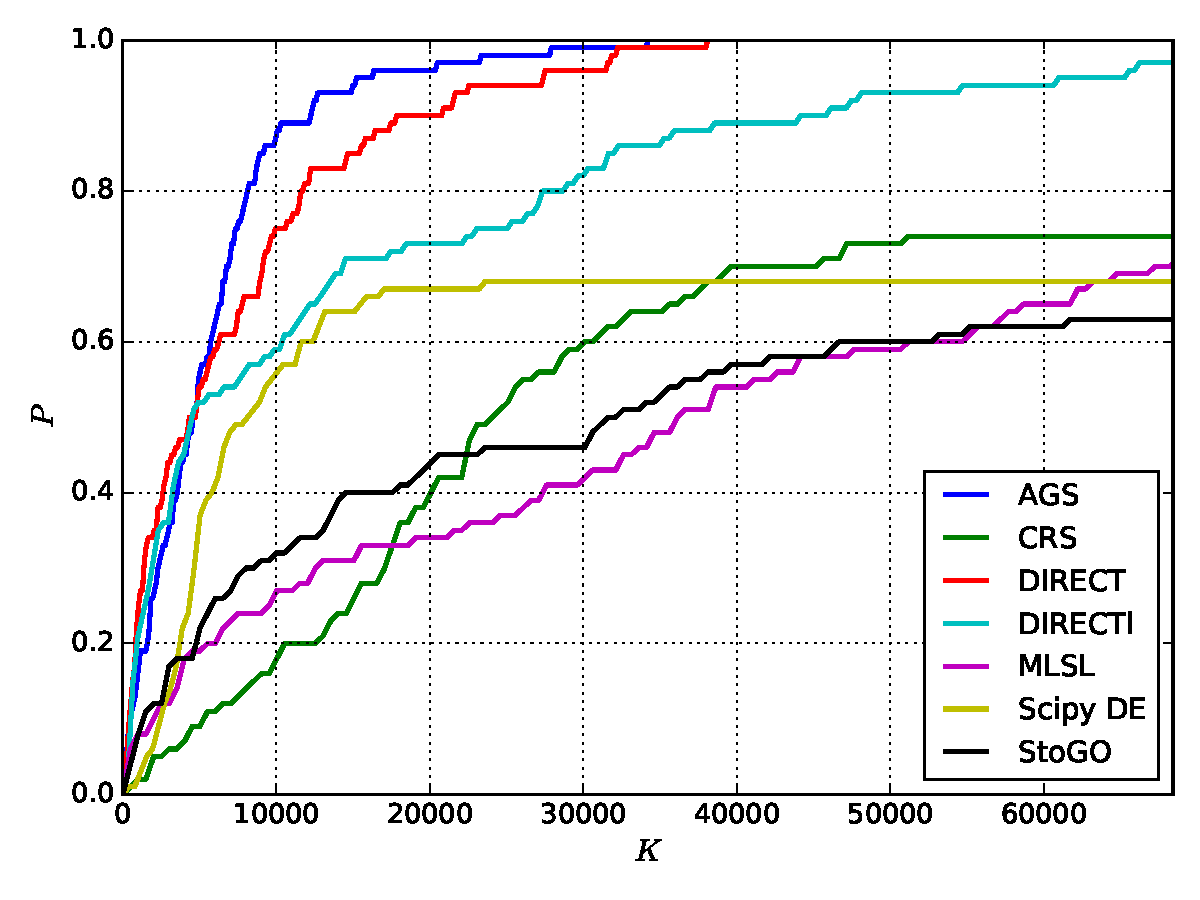
\includegraphics[width=0.95\textwidth]{../experiments_serg_scheme/gklss4d/cmc.pdf}
  \caption{Класс GKLS Simple 4d. Остановка после попадания в окрестность размера $0.0632$}
  \label{fig:}
\end{figure}

\begin{figure}[H]
  \center
  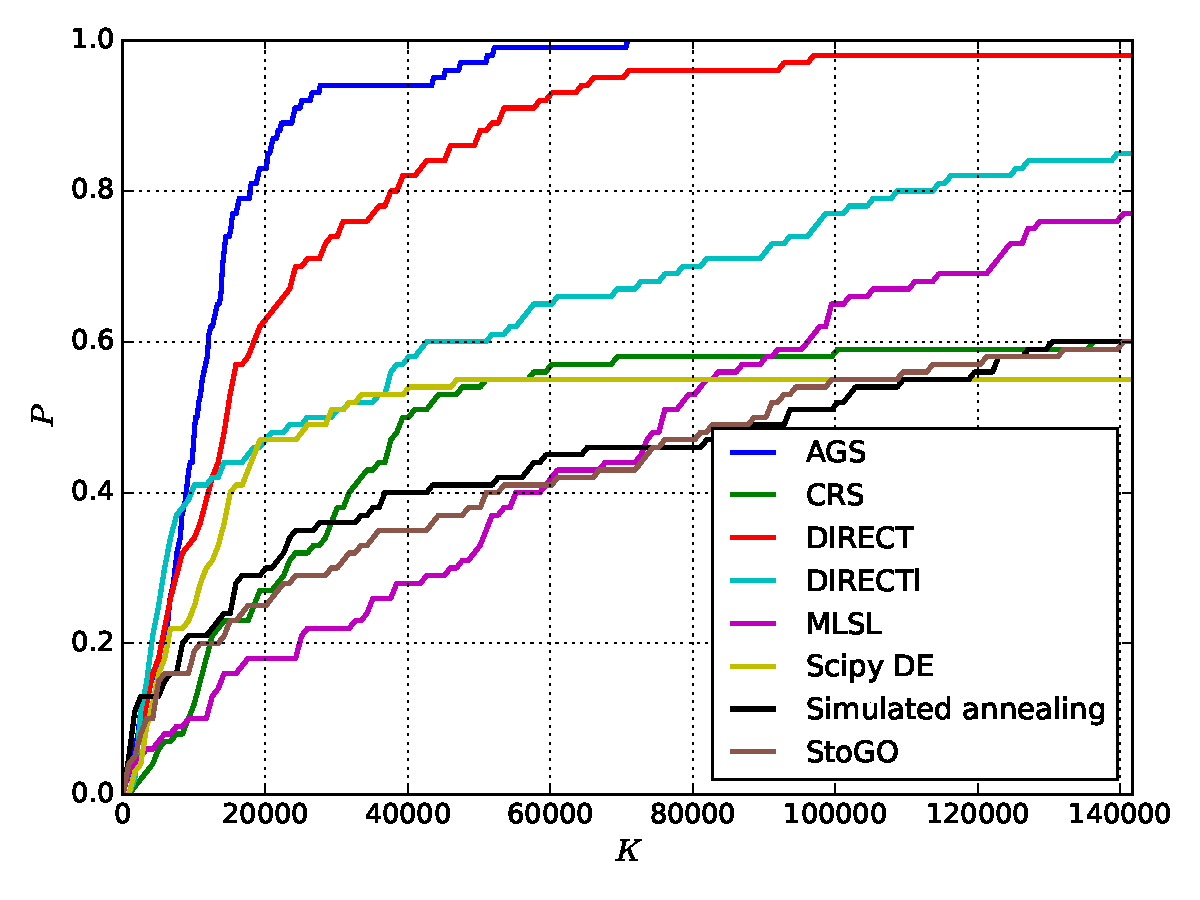
\includegraphics[width=0.95\textwidth]{../experiments_serg_scheme/gklsh4d/cmc.pdf}
  \caption{Класс GKLS Hard 4d. Остановка после попадания в окрестность размера $0.0632$}
  \label{fig:}
\end{figure}

\begin{figure}[H]
  \center
  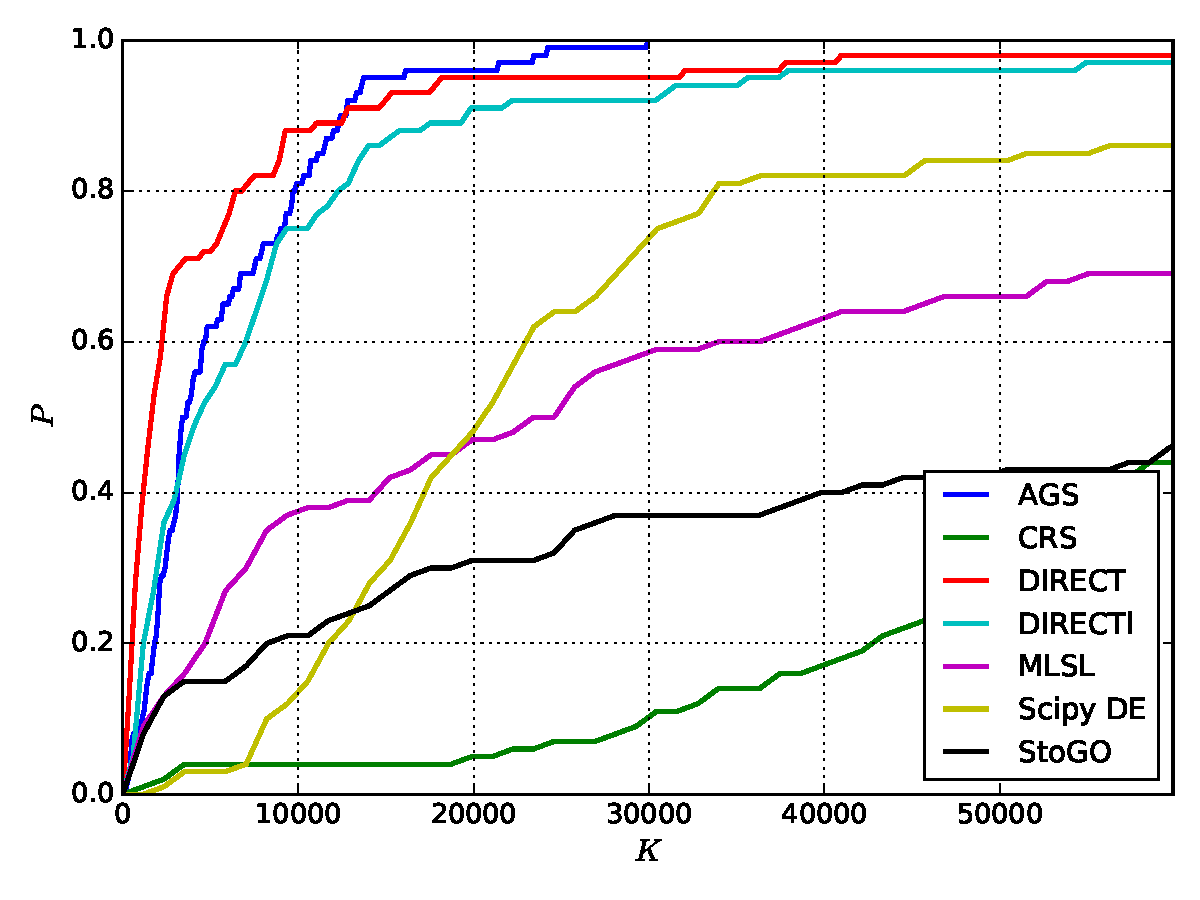
\includegraphics[width=0.95\textwidth]{../experiments_serg_scheme/gklss5d/cmc.pdf}
  \caption{Класс GKLS Simple 5d. Остановка после попадания в окрестность размера $0.0796$}
  \label{fig:}
\end{figure}

\begin{figure}[H]
  \center
  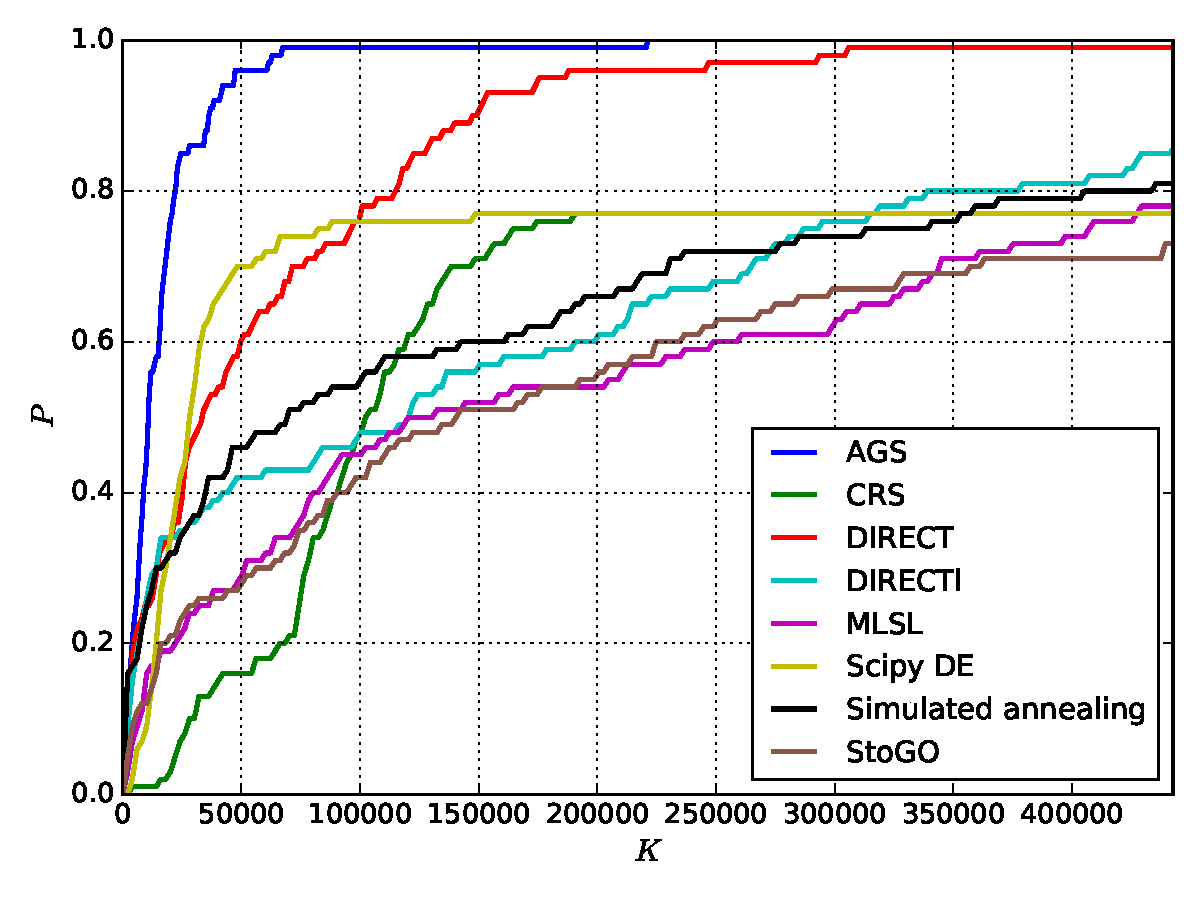
\includegraphics[width=0.95\textwidth]{../experiments_serg_scheme/gklsh5d/cmc.pdf}
  \caption{Класс GKLS Hard 5d. Остановка после попадания в окрестность размера $0.0796$}
  \label{fig:}
\end{figure}

\end{document}
